%% Be sure to check spelling!
%% Put your name and the proper due date in place!
%% Copy the lstlisting and figure code as many times as you need
%% Be sure to put in your own file names if appropriate
%% Note that the \epsfig commands are currently commented out - until the
%%%% files exist, processing this code without them will result in an error
%%%% so leave the comments until you have created the graphics files!
\documentclass{article}
\usepackage{amsmath} % loads AMS-Math package
\usepackage{epsfig} % allows PostScript files
\usepackage{listings} % allows lstlisting environment
\usepackage{moreverb} % allows listinginput environment
\usepackage{vmargin} % allows better margins
\usepackage{graphicx} %allows importing images
\usepackage{placeins}
\usepackage{caption}
\setpapersize{USletter} % sets the paper size
\setmarginsrb{1in}{0.5in}{1in}{0.2in}{12pt}{11mm}{0pt}{11mm} %sets margins 
\begin{document}
\begin{center}
\rule{6.5in}{0.5mm}\\˜\\
{\bf \large ME 334L -- Fall 2014}\\˜\\
{\huge \bf Magnetic Levitation Project}\\˜\\
Justin Palpant (jbp25)\\
Lab Section 02L, Thursday 3:05-5:30\\
December 5, 2014\\˜\\
{\small I understand and have adhered to all the tenets of the Duke
 Community Standard in completing every part of this assignment. I
 understand that a violation of any part of the Standard on any part
 of this assignment can result in failure of this assignment, failure
 of this course, and/or suspension from Duke University.} 
%% YOU WILL SIGN THE DOCUMENT HERE
˜\\˜\\˜\\˜\\
\rule{6.5in}{0.5mm}\\
\end{center}
\tableofcontents
\listoffigures
\pagebreak
\section{Abstract}
The goal of this lab experiment was to implement a form of feedback control of a magnetic levitation device to allow it to control the vertical position of a metal ball according to a control signal.  For our purposes, we wanted to be able to track a variety of control signals, included but not limited to a constant input, a step input, a series of steps in the form of a pulse train, a series of step inputs of randomly generated height, and a sinusoidal input.  We elected to implement a PID controller with a unity gain feedback system which measures the vertical position of the ball via a visual sensor.  In order to tune the gains of this PID controller to make the system stable, we first used the Ziegler-Nichols tuning method to find initial guesses for our gain values which we expected to be near the gains which would result in our desired system response.  Then we manually tuned the gains in small increments while visually inspecting the response until the system responded as desired.  After finding these gains and implementing the various input signals, we found that the PID controller succeeded in maintaining stability with no visible vertical oscillation for constant input and also managed to track each of the reference signals we applied to it.  There was a smaller range of stability than expected, especially with the step and sine input signals, which we attribute largely to the fact that the PID controller does not account for the variation in the magnetic field due to height prior to making its corrections.  We also had an unexpected constant steady state error in response to a constant input, possibly due to the fact that the integral gain of the PID controller had a saturation value, limiting its maximum effect on the system.  We could affect the steady state error and the stable range at the cost of a less desirable system response.  To improve our setup, we would attempt to account more accurately for the physical model of the system, attempt other gain settings to achieve a larger stable range (understanding that any changes will also affect the system response), and possibly recommend implementing a more complicated control system involving predictive control in addition to the reactive control of the PID system.\\
\section{Introduction and Theory}
Our control of the magnetic levitation device was to be based on principles of feedback control of the dynamic system.  To start, we chose to model the system we would be controlling mathematically.  This involved deriving the functions that goverened each step of the system.  Our control of the system consisted of a computer controlled voltage output to an electromagnet.  The electromagnet was assumed to be ohmic, meaning the current through the magnet was related to the voltage according to Ohm's law:The electromagnet exerted a force on a ball, which was related to the current through the electromagnet and the distance of the ball to the magnet. The force on the ball affected the ball's position according to Newton's laws of motion.  Then, the ball position was converted to a voltage measured by the computer via a position sensor which output a voltage which was linear with respect to the difference between the ball's current position and the neutral position.  All together, this system model yields the following five equations: 
\begin{center}
\begin{align}
V_{out} &= V_{set}\\
I_{mag} &= \frac{V_{out}}{R} + I_0\\
F_{ball} &= mg - \frac{I_{mag}^2}{X^2}\\
m\ddot{X} &= F_{ball}\\
V_{meas} &= \lambda(X - X_0)\
\end{align}
\end{center}

These five equations compose the mathematical model of our system.  In this model there are several unknown constants: $I_0$, $R$, $m$, $X_0$, and $\lambda$.  If we had wanted to leverage the system model to create our controller, we would have needed to find these constants.   It is also worth noting that these equations are coupled and nonlinear, which makes them difficult to solve analytically, but would not present a problem for Simulink, which is numerical and iterative.

However, feedback control does not necessarily require knowledge of the system being controlled.  In fact, we chose to use a method of control which only requires measuring the input voltage from the sensor and having control over the output voltage.  This method, PID control, involves calculating the difference between these two values to find the error signal, then combining the error signal, the derivative of the error signal, and the integral of past error, each with a different gain, and using that as the output signal:
\begin{center}
\begin{align}
Error(E) &= V_{set} - V_{meas}\\
V_{out} &= K_p * E + K_i * \int{E} + K_d * \dot{E}
\end{align}
\end{center}

With this, the system needs only the voltage from the sensor and the desired voltage setting to calculate the output voltage.  While this type of controller does not take advantage of all of the available information, it is commonly used and can be expected, in our situation, to be able to stabilize the system if appropriate gain values, $K_p$, $K_i$, and $K_d$ are found.  In our lab, we will design a PID controller in Simulink, connect it to a ControlDesk layout which will be able to control the PID gains as well as the value of the input signal to the system, and then tune the PID controller to maintain the vertical position of the ball stably for various reference signals.

\section{Procedure}
The lab began with the design of our Simulink model and ControlDesk layout.  Our Simulink model was a basic unity-gain feedback control model - we measured the output voltage of the system using the dSPACE R1104 data acquisition board, calculated the difference between that position and our reference signal, passed the error through a PID block of our own creation, and sent the output of the PID block to the magnetic levitation device using the dSPACE board again.  A screenshot of the Simulink model can be found as figure~\ref{fig:sim} and a screenshot of the inside of the PID controller is figure ~\ref{fig:pid}.  The Simulink controller also included a multiport switch controlling which of our reference inputs would be used, as well as all five of the possible reference inputs: constant, random step, sine, pulse train, and input from an extra input of our own design - a voltage measured from an external circuit designed to convert the height of an object above the circuit to a voltage, measurable by the dSPACE control desk.  The construction of this circuit will be described later.

Additionally, we designed a ControlDesk layout, consisting of sliders and numeric inputs for each gain value, as well as for the amplitude and frequency of each signal for which these values were relevant, two numeric indicators for output voltage of Simulink and the voltage measured by the ball detector, and a graphical indicator for the setpoint voltages and the measured voltages.  The layout is shown as figure~\ref{fig:controldesk}.

With the Simulink and the dSPACE connected and running to control the device, we needed to tune our PID gains so that the system would remain stable and have the desired system response.  To do so, we used two methods - the Ziegler-Nichols tuning method, and manual, iterative tuning.  The Ziegler-Nichols tuning method involves beginning with all gains at zero and increasing the proportional gain until the system begins to oscillate.  At this point, when oscillations are stable, the period of the oscillation is measured in seconds.  When combined with the gain at which this occurred, gains can be calculated for proportional, proportional-integral, or proportional-integral-derivative control.  The calculated gains are designed to have the effect of causing a large overshoot and quarter-wave decay, which causes the amplitude of the oscillations to decay to 75\% in each oscillation.  The values we found for this tuning process are included in the results section.

Following Ziegler-Nichols tuning, we found that the integral gain $K_i$ was too large for the system to be stable.  We adjusted the gains incrementally, making small changes to each gain and observing the system response until the system had the desired response.  The system response and the gains we found are included in the results section as well. 

With our system tuned, all that remained was to implement the final input signal.  For this, we wanted to be able to control the height of the ball by moving our hands.  To do so, we used an Arduino and an ultrasonic distance sensor which would query the distance to the nearest object and, if it was close enough, output a PWM voltage signal proportional to the object's distance.  However, when a slow PWM signal is sampled at a rapid rate, it results in alternating high and low signals - this would be a bad input to the magnetic levitation device.  The PWM signal from the Arduino is known to have a frequency of 490Hz - compared to the Simulink sample speed of 1kHz, this is very slow. As a result, the PWM signal would be smooth, averaged using a lowpass RC filter.  If the time constant of the RC filter is long enough, the PWM signal is averaged, ideally resulting in a voltage which is constant and can be sampled at any frequency. We chose $R = 4.7k\Omega$ and $C = 4.7\mu F$ for a time constant of 22.09ms, which is longer than the PWM period of 2.04ms by a factor of ten a smoothing we imagined would be sufficient to result in a smooth, easily measured output.

\section{Results and Conclusions}
The first results of this lab were the PID gains found via the Ziegler-Nichols tuning method.  At the point when the oscillation was small and had constant amplitude, we measured the critical gain and the ultimate period to be
\begin{center}
\begin{align*}
K_u &= 2.0 \\
T_p &= 0.2~seconds
\end{align*}
\end{center}
This yields a gain matrix as follows:
\begin{center}
\begin{tabular}{|c|c|c|c|} \hline
Control Type & $K_p$ & $K_i$ & $K_d$ \\ \hline
P & $0.5K_u = 1$ & - & - \\
PI & $0.45K_u = 0.9$ & $\frac{1.2K_p}{T_u} = 5.4$ & - \\
PID & $0.6K_u = 1.2$ & $\frac{2K_p}{T_u} = 12$ & $\frac{K_pT_u}{8} = 0.03$ \\ \hline
\end{tabular}
\end{center}

Since we were working with a PID controller, we used the gains in the last row.  However, these gains were obviously unusable, especially the integral gain $K_i$, which is far too large.  When testing these gains, we noticed that the integral gain dominated the controller.  The behavior that resulted from this was that the ball consistently overcorrected, rising until it left the stable range.  At that point, the controller attempted to release the ball, but due to the increase in strength of the magnetic field near the magnet, the controller could not push the ball away from the magnet.

We imagined that the other two gains, $K_p$ and $K_d$ were nearly correct, however, so be began the process of tuning the system to achieve a desirable system response.  In descending order of importance: we wanted the ball to be stable at the origin (the point where the sensor voltage was zero) and in a range above and below that point; we wanted a quick response to step function that looked to the human eye to be show enough not to be immediate; we wanted to minimized steady state error of a constant input and we wanted to track a sinusoidal input with near-unity gain and minimal phase shift.

We tuned our controller manually based on human intuition of how the response was changing with respect to the changing gains.  We began with the Z-N tuned gains, set $K_i$ to be equal to zero, and then gradually increased each gain.  We increased $K_p$ and $K_i$ by small amounts until the system was nearly stable but had a slight overshoot.  Then, we increased $K_d$ to correct for this overshoot, as increasing the derivative gain helps limit the velocity of the ball.  We found one set of gains but determined that the system response to step input was too slow. To correct that we decreased the derivative gain and the integral gain - decreasing the derivative gain caused an decrease in stability in exchange for a faster response, while decreasing the integral gain caused an increase in the steady-state error for a constant input.  We eventually found the following gains:
\begin{center}
\begin{align*}
K_p &= 2.14\\
K_i &= 1.4*10^{-3}\\
K_d &= 6.5*10^{-2}\\
\end{align*}
\end{center}

With these gains, we analyzed the system response of our controller for each of the criteria we had established at the beginning of the process.  First, we looked at each of our input signals and determined the range of valid values (amplitude and frequency) within which the system would remain stable.  While a larger ranges were considered desirable for our application, what was crucial was that the ranges be significant enough to be noticeable with the naked eye.  We determined the stable ranges for amplitude (in volts) and for frequency (in Hertz) by varying these parameters individually and determining the point of failure, when the system could not remain stable.  We found the following values:

\begin{center}
\begin{tabular}{|c|c|c|} \hline
Input Type & Amplitude (V) & Frequency (Hz) \\ \hline
Constant & [-0.11, 0.15] & -\\
Step & [-0.11, 0.15] & -\\
Pulse Train & [0, 0.04] & [0, 1]\\
Sine & [0, 0.075] & [0, 2]\\ \hline
\end{tabular}
\end{center}

These values show that the system is more able to respond to a sinusoidal input than it is to a step input, as the range of amplitudes and of frequencies is larger for the sine input.  Additionally, both of the ranges of amplitudes for those input signals are smaller than the maximum range of the function - this makes sense, as with those functions the system has to account for additional acceleration, and is less able to maintain stability.  As long as the input parameters were maintained within these ranges, we found that the system could maintain stability.  We then attempted to determine important numerical values relating to the system response, such as the steady-state error for a constant input, the time constant for a step input, and the gain and phase shift for a sinusoidal input.  In order to do this we plotted the input signal and the response signal on the same graph and compared the signals.  Figures~\ref{fig:ss} to~\ref{fig:sine} in section~\ref{sec:fig} show the graphs from which we determined each of our important system response values. 

First, we determined the steady-state error.  In our case, this is directly observable in Figure~\ref{fig:ss} - the steady state error is the difference between the red and green lines, which represent the input signal and the feedback signal.  We had a steady state error of approximately 0.7 volts - this is significant, considering the allowable range for constant input was only [-0.11, 0.15] volts.  This was surprising, because we could expect the integral block to gradually or quickly decrease this error over time.  However, we had specifically decreased the gain of the integral block, in addition to applying a saturation limit (the maximum error the integral block can accumulate).  The product of our saturation limit, 100V, and our $K_i$, 0.0014, is 0.14V.  This is the maximum effect the integral gain can have, and this may not be enough to decrease the error.  This rationale for the large steady state error makes sense, because we found the increasing the integral gain consistently decreased the steady state error.  We also suspect some sort of voltage offset in either our input or output, because this error was noticeable for many signals, include the sine signal, indicating that it is not solely steady state error, but also possibly some kind of bias in our system.

We made the assumption that the system response to the step input would be exponential approach, as one would expect of a first order system.  While our system is not necessarily first order, the observable response to a step input did appear to be exponential approach - there was not visible overshoot or oscillation on our output graph.  This means that an appropriate way to determine the speed of the system would be to determine the system's time constant.  To determine the time constant, we found on the step input the point at which the rise started and the point at which, to the eye, the output had reached a steady state.  We determined that the time difference between these points would be approximately three time constants, as after three time constants a first order system will have moved 95.02\% of the distance between the start and final values.  We measured a response time of approximately 0.15 seconds from Figure~\ref{fig:tc}, indicating a time constant $\tau = 0.05 s$, or 50 milliseconds.  This fractional-second response time is one of the traits we most wanted in our system - it is short enough that when a step input is applied, response seems quick and sharp to the human eye.

Lastly we determined the gain and phase shift of the system response to a sinusoidal input.  From the graph in Figure~\ref{fig:sine}, it is clear that there is not an appreciable phase shift, or not one which could be easily measured - there is perhaps some small time delay, but with the data available we determined that a phase shift in milliseconds would be too small to be consistently measured, and we did not calculate it.  The gain, however, can be calculated - it is easily noticeable that the output signal is larger than the input signal (they are also offset - again, due likely to some inherent voltage bias in the system).  This means that the gain will be greater than one.  We find the gain as follows:
\begin{center}
\begin{align*}
G &= \frac{A_{vo}}{A_{vi}} \\
G_{dB} &= 20\log(G)
\end{align*}
\end{center}

We measured $A_{vo} = 0.16 V$ and $A_{vi} = 0.1 V$, yielding
\begin{center}
\begin{align*}
G &= \frac{0.16}{0.1} = 1.6 \\
G_{dB} &= 20\log(1.6) = 9.4
\end{align*}
\end{center}

After analyzing the response to these standard inputs, we tested our hand-control input and found that while the system was functional, it was less responsive to hand height change than to the other input signals.  It also had significant noise in the response - while holding the hand steady, the ball would oscillate or bounce noticeably.  This means that the voltage output of the hand-measuring circuit was not constant - a result that, while expected, was disappointing.  It may have been that the smoothing effect of the RC lowpass filter was not sufficient, and that oscillations of the low-frequency PWM wave were maintained in the voltage output.  This is the most likely scenario, because the time constant of the RC filter, 22.09 ms, is short enough that our circuit simulation indicated there would be oscillation due to the PWM input.  A longer time constant on the filter may have alleviated this, at the cost of a slower response to the changes in the height being measured.  It could also have been due to significant variation in measurement of the hand height - the system has limited precision and may have measured a variation of several centimeters even while the hand being detected was not moving.  

There are several changes which could be recommended to improve our system.  In order to improve the stable range for all functions, the Simulink model could be improved by leveraging what is known about the physical model.  The convenience of PID control is that this is not necessary, but including some simply physical information could improve the control of the system, for instance, knowing that the magnetic field strength decays with the square of the distance from the magnet would make the system more able to resist moving into regions where it will not be able to control the ball. It would also be able to control the ball in a larger range of regions because it would use more of the system's output.  Currently, the system output voltage remains less than one volt in magnitude, but it has a possible range of plus-or-minus 10 volts - using more of that range would allow the ball to be controlled at greater extremes.

Alternatively, a predictive controller which takes into account not only current and past error but also future error and anticipates future voltage setting could, if computationally possible, result in good system response.  However, that is outside of the realm of the feedback control we have learned in the course.\\
\section{Figures}
\label{sec:fig} 
\FloatBarrier
\begin{figure}
\centering
\includegraphics[width=8.5in]{Simulink.jpg}
\caption{Simulink model}
\label{fig:sim}
\end{figure}

\begin{figure}
\centering
\includegraphics[width=6.5in]{PIDBlock.jpg}
\caption{PID Control block Simulink model}
\label{fig:pid}
\end{figure}

\begin{figure}
\centering
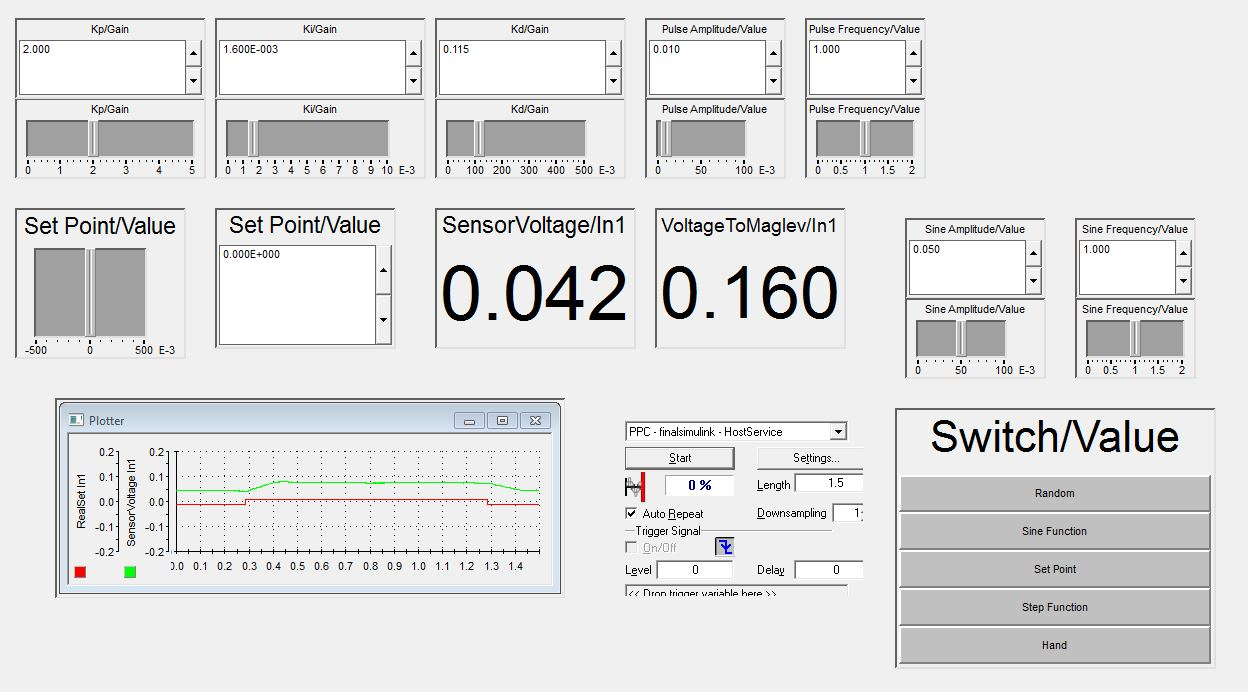
\includegraphics[width=8.5in]{layout.jpg}
\caption{ControlDesk Layout}
\label{fig:controldesk}
\end{figure}

\begin{figure}
\centering
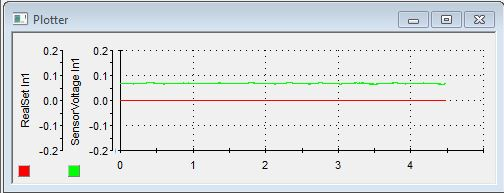
\includegraphics[width=8.5in]{Steadystate.jpg}
\caption{Plot showing steady state error for constant input}
\label{fig:ss}
\end{figure}

\begin{figure}
\centering 
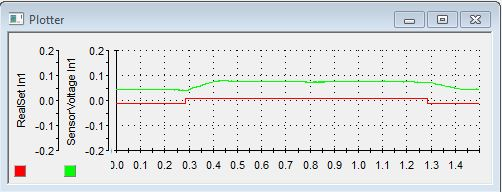
\includegraphics[width=8.5in]{Timeconstant.jpg}
\caption{Plot showing system response and time constant for step input}
\label{fig:tc}
\end{figure}

\begin{figure}
\centering 
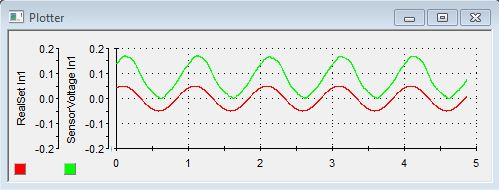
\includegraphics[width=8.5in]{Sine.jpg}
\caption{Plot showing system response, gain and phase shift for sine input}
\label{fig:sine}
\end{figure}
\end{document}